\documentclass[12pt]{scrartcl}
\usepackage{config}
\usepackage{minted}

%\newcommand\mrh{\color{white}\bfseries}
\newcommand\mrc[1]{\begin{tabular}{@{}l@{}} #1 \end{tabular}}
\setlength\arrayrulewidth{0.8pt}

\usemintedstyle{pastie}

\begin{document}
    \hh{Arbol-stían}
    
    
    \vspace{10pt}

    
    \hh{Problema}
    
        Te es dado un entero $N$ y $N - 1$ aristas bidireccionales con peso. Estas aristas conectan $N$ vértices de tal forma que exista un camino\footnote{Un camino se define como una secuencia de vértices, tal que para cualesquiera dos vértices consecutivos existe una arista que los conecta.} entre cualesquiera dos vértices (es decir forman un árbol). Para todos los caminos, definimos su peso como el producto de la cantidad de aristas en él, y el {\bfseries máximo común divisor} de cada uno de los pesos de las aristas en el camino en el camino. Determina el camino simple (que no repite aristas) con peso máximo.
    
    \hh{Detalles de Implementación}

        Debes implementar la función \textit{Arbolstian()}. Esta función recibe un entero $N$ y 3 vectores, $u, v$ y $w$  con $N - 1$ elementos.. Para cada $0 \le i \le N - 2$, $u[i]$ y $v[i]$ son los vértices que se conectan con la arista $i$, y $w[i]$ su peso. Esta función debe regresar un entero, el peso máximo en camino del árbol.
        La función se vería así:

\begin{minted}{c++}
#include <bits/stdc++.h>
using namespace std;

long long int Arbolstian(int N, vector<int> u, vector<int> v, vector<int> w) {
    // Implementa esta función.
}
\end{minted}

    El evaluador llamará la función \textbf{múltiples} veces por caso de prueba.

    \hh{Ejemplos}
    
        {\itshape Ejemplo 1:}
        \begin{itemize}
            \item El evaluador llama la función 
            \begin{center}
                \textit{Arbolstian(6, \{0, 0, 0, 2, 3\}, \{1, 2, 3, 4, 5\}, \{2, 2, 4, 2, 4\})}
            \end{center}
            el árbol en este ejemplo es el siguiente:
            
            \begin{center}
                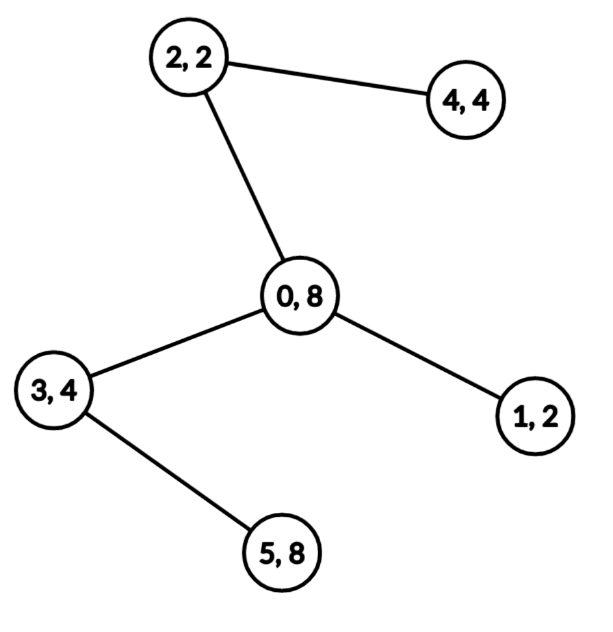
\includegraphics[scale=0.2]{ej1.png}
            \end{center}
            \item Los caminos posibles y sus pesos en este árbol son:
            \begin{center}
                \begin{tabular}{|c||c|c|c|c|c|c|}
                    \hline
                     $dist(a, b)$ & 0 & 1 & 2 & 3 & 4 & 5 \\
                     \hline
                     \hline
                     0 & 0 & 2 & 2 & 4 & 4 & 8 \\
                     \hline
                     1 & 2 & 0 & 4 & 4 & 6 & 6 \\
                     \hline
                     2 & 2 & 4 & 0 & 4 & 2 & 6 \\
                     \hline
                     3 & 4 & 4 & 4 & 0 & 6 & 4 \\
                     \hline
                     4 & 4 & 6 & 2 & 6 & 0 & 8 \\
                     \hline
                     5 & 8 & 6 & 6 & 4 & 8 & 0 \\ 
                     \hline
                \end{tabular}
            \end{center}
            \item La respuesta correcta es $8$.
        \end{itemize}

        {\itshape Ejemplo 2:}
        \begin{itemize}
            \item El evaluador llama la función 
            \begin{center}
                \textit{Arbolstian(9, \{0, 1, 2, 3, 4, 5, 6, 7\}, \{1, 2, 3, 4, 5, 6, 7, 8\}, \{3, 3, 5, 2, 7, 7, 3, 2\})}
            \end{center}
            el árbol en este ejemplo es el siguiente:
            \begin{center}
                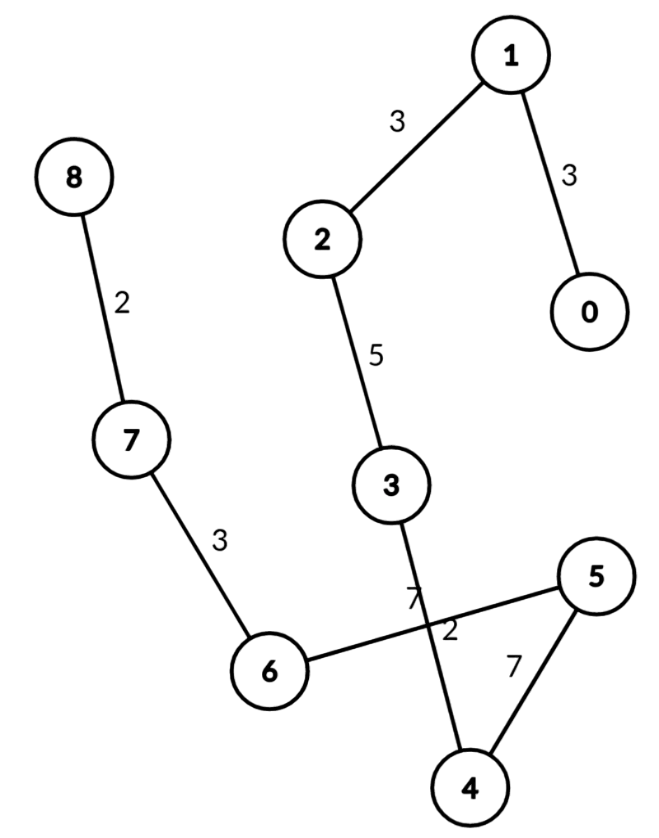
\includegraphics[scale=0.2]{ej2.png}
            \end{center}
            \item La respuesta correcta es $14$.
        \end{itemize}
        

    \hh{Consideraciones}
        \begin{itemize}
            \item $1 \le N \le 2\times10^5$.
            \item Los vectores $u, v$ y $w$ tendrán exactamente $N - 1$ elementos.
            \item Para cada $0 \le i \le N - 2$, se cumple que $0 \le u[i] \neq v[i] < N$. 
            \item Para cada $0 \le i \le N - 2$, se cumple que $1 \le w[i] \le 10^6$.
            \item Se garantiza que el grafo formado por las aristas es un árbol.
            \item Sea $S_N$ la suma de todos los valores de $N$ sobre todas las llamadas a la función. Se garantiza que $S_N \le 2\times 10^5$.
        \end{itemize}
    
    \hh{Subtareas}


    \begin{itemize}
        \item (3 puntos) $N, S_N \le 2000$.
        \item (9 puntos) Para todo $0 \le i \le N - 1$, se cumple que $w[i] = 1$.
        \item (11 puntos) Para todo $0 \le i \le N - 2$, el peso de la arista $w[i]$ es 1.
        \item (22 puntos) Para todo $0 \le i \le N - 2$, se cumple que $w[i]$ es una potencia de 2.
        \item (22 puntos) Para todo $0 \le i \le N - 2$, se cumple que $u[i] = i, v[i] = i + 1$.
        \item (33 puntos) Sin restricciones adicionales.
    \end{itemize}
\end{document}
